\documentclass[prd,twocolumn]{revtex4}

\pdfoutput=1

\usepackage{graphicx}
\usepackage{dcolumn}
\usepackage{bm}
\usepackage{amssymb,amsmath,bm}  
\usepackage{color}
\usepackage{hyperref}
\usepackage{multirow}
\usepackage[utf8]{inputenc}
\usepackage{balance}
\usepackage{enumitem}
\usepackage{lipsum}
\newcommand{\uKam}{\mu\text{K-arcmin}}
\newcommand{\nv}{\hat{\bf n}}
\newcommand{\jcap}{JCAP}
\newcommand{\mnras}{MNRAS}
\newcommand{\aap}{A\&A}
\newcommand{\aaps}{A\&AS}
\newcommand{\apjs}{ApJS}
\newcommand{\apjl}{ApJL}
\newcommand{\aj}{Astron. Journal}
\newcommand{\pasp}{Publications of the ASP}
\newcommand{\nar}{New Astronomy Review}
\newcommand{\procspie}{Proceedings of the SPIE}


\begin{document}
\title{Calibrating photometric redshifts with intensity mapping observations}
\author{All of us$^1$}
\affiliation{$^{1}$University of Wherever}

\begin{abstract}
  \lipsum[0]
\end{abstract}

  \date{\today}
  \maketitle

\section{Introduction}\label{sec:intro}
  \lipsum[1]
  
\section{Formalism}\label{sec:method}
  \subsection{Clustering-based photo-$z$ calibration}\label{ssec:method.clustred}
    \lipsum[2]
  \subsection{Intensity mapping}\label{ssec:method.imap}
    \lipsum[3]
  \subsection{Forecasting formalism}\label{ssec:method.fisher}
    \lipsum[4]

\section{Results} \label{sec:results}
  \subsection{Baseline forecasts} \label{ssec:results.baseline}
    \lipsum[5]
  \subsection{Dependence on experimental parameters} \label{ssec:results.params}
    \lipsum[6]
  \subsection{Outliers and non-Gaussian photo-$z$s} \label{ssec:results.outliers}
    \lipsum[7]
  \subsection{Non-parametric redshift distributions} \label{ssec:results.nonpar}
    \lipsum[8]

  \begin{figure}
    \centering
    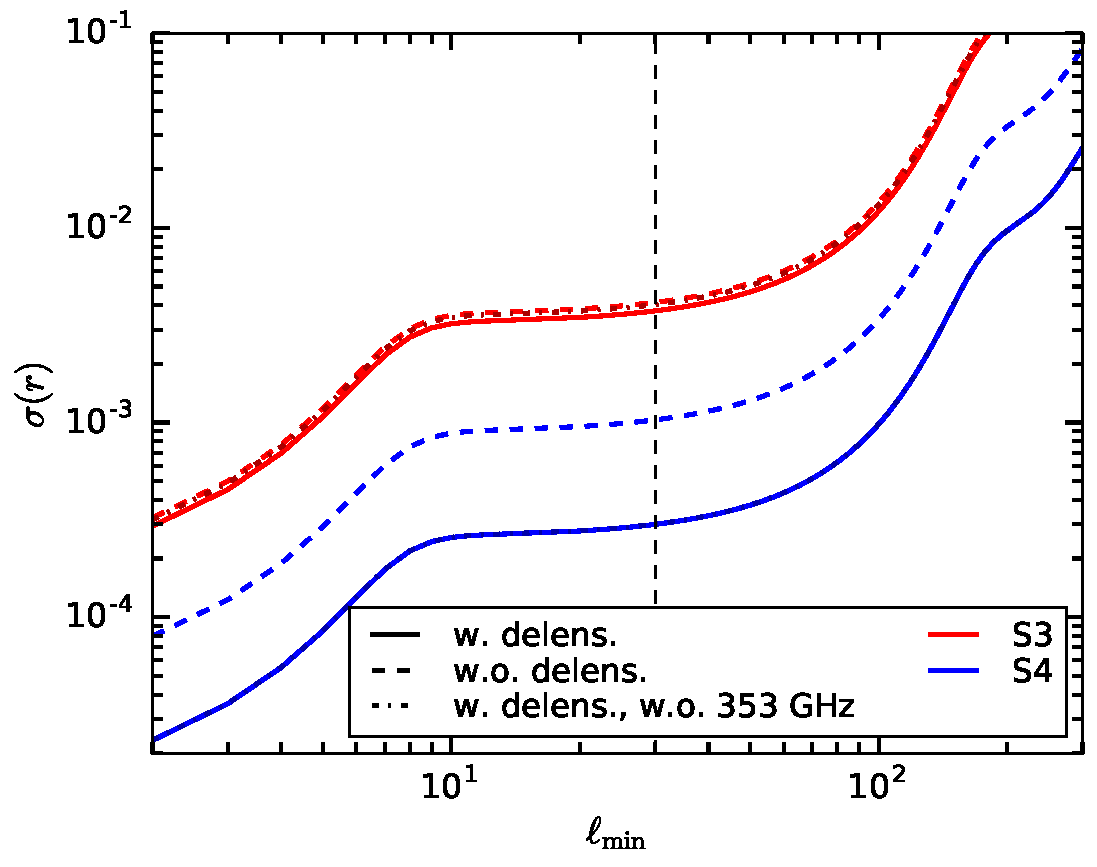
\includegraphics[width=0.49\textwidth]{fisher_lmin}
    \caption{}
    \label{fig:fisher}
  \end{figure}

\section{Discussion}\label{ssec:discuss}
  \lipsum[9]

\section*{Acknowledgments}
  We thank Odin the almighty for useful comments and discussions.
 
\bibliography{paper}

\appendix
\begin{widetext}
  \section{Appendix}\label{app:app}
    \lipsum[10]
\end{widetext}

\end{document}
